\documentclass{report}

%%%%%%%%%%%%%%%%%%%%%%%%%%%%%%%%%
% PACKAGE IMPORTS
%%%%%%%%%%%%%%%%%%%%%%%%%%%%%%%%%


\usepackage[tmargin=2cm,rmargin=1in,lmargin=1in,margin=0.85in,bmargin=2cm,footskip=.2in]{geometry}
\usepackage{amsmath,amsfonts,amsthm,amssymb,mathtools}
\usepackage[varbb]{newpxmath}
\usepackage{xfrac}
\usepackage[makeroom]{cancel}
\usepackage{mathtools}
\usepackage{bookmark}
\usepackage{enumitem}
\usepackage{hyperref,theoremref}
\hypersetup{
	pdftitle={Assignment},
	colorlinks=true, linkcolor=doc!90,
	bookmarksnumbered=true,
	bookmarksopen=true
}
\usepackage[most,many,breakable]{tcolorbox}
\usepackage{xcolor}
\usepackage{varwidth}
\usepackage{varwidth}
\usepackage{etoolbox}
%\usepackage{authblk}
\usepackage{nameref}
\usepackage{multicol,array}
\usepackage{tikz-cd}
\usepackage[ruled,vlined,linesnumbered]{algorithm2e}
\usepackage{comment} % enables the use of multi-line comments (\ifx \fi) 
\usepackage{import}
\usepackage{xifthen}
\usepackage{pdfpages}
\usepackage{transparent}

\newcommand\mycommfont[1]{\footnotesize\ttfamily\textcolor{blue}{#1}}
\SetCommentSty{mycommfont}
\newcommand{\incfig}[1]{%
    \def\svgwidth{\columnwidth}
    \import{./figures/}{#1.pdf_tex}
}

\usepackage{tikzsymbols}
\renewcommand\qedsymbol{$\Laughey$}


%\usepackage{import}
%\usepackage{xifthen}
%\usepackage{pdfpages}
%\usepackage{transparent}


%%%%%%%%%%%%%%%%%%%%%%%%%%%%%%
% SELF MADE COLORS
%%%%%%%%%%%%%%%%%%%%%%%%%%%%%%



\definecolor{myg}{RGB}{56, 140, 70}
\definecolor{myb}{RGB}{45, 111, 177}
\definecolor{myr}{RGB}{199, 68, 64}
\definecolor{mytheorembg}{HTML}{F2F2F9}
\definecolor{mytheoremfr}{HTML}{00007B}
\definecolor{mylenmabg}{HTML}{FFFAF8}
\definecolor{mylenmafr}{HTML}{983b0f}
\definecolor{mypropbg}{HTML}{f2fbfc}
\definecolor{mypropfr}{HTML}{191971}
\definecolor{myexamplebg}{HTML}{F2FBF8}
\definecolor{myexamplefr}{HTML}{88D6D1}
\definecolor{myexampleti}{HTML}{2A7F7F}
\definecolor{mydefinitbg}{HTML}{E5E5FF}
\definecolor{mydefinitfr}{HTML}{3F3FA3}
\definecolor{notesgreen}{RGB}{0,162,0}
\definecolor{myp}{RGB}{197, 92, 212}
\definecolor{mygr}{HTML}{2C3338}
\definecolor{myred}{RGB}{127,0,0}
\definecolor{myyellow}{RGB}{169,121,69}
\definecolor{myexercisebg}{HTML}{F2FBF8}
\definecolor{myexercisefg}{HTML}{88D6D1}


%%%%%%%%%%%%%%%%%%%%%%%%%%%%
% TCOLORBOX SETUPS
%%%%%%%%%%%%%%%%%%%%%%%%%%%%

\setlength{\parindent}{1cm}
%================================
% THEOREM BOX
%================================

\tcbuselibrary{theorems,skins,hooks}
\newtcbtheorem[number within=section]{Theorem}{Theorem}
{%
	enhanced,
	breakable,
	colback = mytheorembg,
	frame hidden,
	boxrule = 0sp,
	borderline west = {2pt}{0pt}{mytheoremfr},
	sharp corners,
	detach title,
	before upper = \tcbtitle\par\smallskip,
	coltitle = mytheoremfr,
	fonttitle = \bfseries\sffamily,
	description font = \mdseries,
	separator sign none,
	segmentation style={solid, mytheoremfr},
}
{th}

\tcbuselibrary{theorems,skins,hooks}
\newtcbtheorem[number within=chapter]{theorem}{Theorem}
{%
	enhanced,
	breakable,
	colback = mytheorembg,
	frame hidden,
	boxrule = 0sp,
	borderline west = {2pt}{0pt}{mytheoremfr},
	sharp corners,
	detach title,
	before upper = \tcbtitle\par\smallskip,
	coltitle = mytheoremfr,
	fonttitle = \bfseries\sffamily,
	description font = \mdseries,
	separator sign none,
	segmentation style={solid, mytheoremfr},
}
{th}


\tcbuselibrary{theorems,skins,hooks}
\newtcolorbox{Theoremcon}
{%
	enhanced
	,breakable
	,colback = mytheorembg
	,frame hidden
	,boxrule = 0sp
	,borderline west = {2pt}{0pt}{mytheoremfr}
	,sharp corners
	,description font = \mdseries
	,separator sign none
}

%================================
% Corollery
%================================
\tcbuselibrary{theorems,skins,hooks}
\newtcbtheorem[number within=section]{Corollary}{Corollary}
{%
	enhanced
	,breakable
	,colback = myp!10
	,frame hidden
	,boxrule = 0sp
	,borderline west = {2pt}{0pt}{myp!85!black}
	,sharp corners
	,detach title
	,before upper = \tcbtitle\par\smallskip
	,coltitle = myp!85!black
	,fonttitle = \bfseries\sffamily
	,description font = \mdseries
	,separator sign none
	,segmentation style={solid, myp!85!black}
}
{th}
\tcbuselibrary{theorems,skins,hooks}
\newtcbtheorem[number within=chapter]{corollary}{Corollary}
{%
	enhanced
	,breakable
	,colback = myp!10
	,frame hidden
	,boxrule = 0sp
	,borderline west = {2pt}{0pt}{myp!85!black}
	,sharp corners
	,detach title
	,before upper = \tcbtitle\par\smallskip
	,coltitle = myp!85!black
	,fonttitle = \bfseries\sffamily
	,description font = \mdseries
	,separator sign none
	,segmentation style={solid, myp!85!black}
}
{th}


%================================
% LENMA
%================================

\tcbuselibrary{theorems,skins,hooks}
\newtcbtheorem[number within=section]{Lenma}{Lenma}
{%
	enhanced,
	breakable,
	colback = mylenmabg,
	frame hidden,
	boxrule = 0sp,
	borderline west = {2pt}{0pt}{mylenmafr},
	sharp corners,
	detach title,
	before upper = \tcbtitle\par\smallskip,
	coltitle = mylenmafr,
	fonttitle = \bfseries\sffamily,
	description font = \mdseries,
	separator sign none,
	segmentation style={solid, mylenmafr},
}
{th}

\tcbuselibrary{theorems,skins,hooks}
\newtcbtheorem[number within=chapter]{lenma}{Lenma}
{%
	enhanced,
	breakable,
	colback = mylenmabg,
	frame hidden,
	boxrule = 0sp,
	borderline west = {2pt}{0pt}{mylenmafr},
	sharp corners,
	detach title,
	before upper = \tcbtitle\par\smallskip,
	coltitle = mylenmafr,
	fonttitle = \bfseries\sffamily,
	description font = \mdseries,
	separator sign none,
	segmentation style={solid, mylenmafr},
}
{th}


%================================
% PROPOSITION
%================================

\tcbuselibrary{theorems,skins,hooks}
\newtcbtheorem[number within=section]{Prop}{Proposition}
{%
	enhanced,
	breakable,
	colback = mypropbg,
	frame hidden,
	boxrule = 0sp,
	borderline west = {2pt}{0pt}{mypropfr},
	sharp corners,
	detach title,
	before upper = \tcbtitle\par\smallskip,
	coltitle = mypropfr,
	fonttitle = \bfseries\sffamily,
	description font = \mdseries,
	separator sign none,
	segmentation style={solid, mypropfr},
}
{th}

\tcbuselibrary{theorems,skins,hooks}
\newtcbtheorem[number within=chapter]{prop}{Proposition}
{%
	enhanced,
	breakable,
	colback = mypropbg,
	frame hidden,
	boxrule = 0sp,
	borderline west = {2pt}{0pt}{mypropfr},
	sharp corners,
	detach title,
	before upper = \tcbtitle\par\smallskip,
	coltitle = mypropfr,
	fonttitle = \bfseries\sffamily,
	description font = \mdseries,
	separator sign none,
	segmentation style={solid, mypropfr},
}
{th}


%================================
% CLAIM
%================================

\tcbuselibrary{theorems,skins,hooks}
\newtcbtheorem[number within=section]{claim}{Claim}
{%
	enhanced
	,breakable
	,colback = myg!10
	,frame hidden
	,boxrule = 0sp
	,borderline west = {2pt}{0pt}{myg}
	,sharp corners
	,detach title
	,before upper = \tcbtitle\par\smallskip
	,coltitle = myg!85!black
	,fonttitle = \bfseries\sffamily
	,description font = \mdseries
	,separator sign none
	,segmentation style={solid, myg!85!black}
}
{th}



%================================
% Exercise
%================================

\tcbuselibrary{theorems,skins,hooks}
\newtcbtheorem[number within=section]{Exercise}{Exercise}
{%
	enhanced,
	breakable,
	colback = myexercisebg,
	frame hidden,
	boxrule = 0sp,
	borderline west = {2pt}{0pt}{myexercisefg},
	sharp corners,
	detach title,
	before upper = \tcbtitle\par\smallskip,
	coltitle = myexercisefg,
	fonttitle = \bfseries\sffamily,
	description font = \mdseries,
	separator sign none,
	segmentation style={solid, myexercisefg},
}
{th}

\tcbuselibrary{theorems,skins,hooks}
\newtcbtheorem[number within=chapter]{exercise}{Exercise}
{%
	enhanced,
	breakable,
	colback = myexercisebg,
	frame hidden,
	boxrule = 0sp,
	borderline west = {2pt}{0pt}{myexercisefg},
	sharp corners,
	detach title,
	before upper = \tcbtitle\par\smallskip,
	coltitle = myexercisefg,
	fonttitle = \bfseries\sffamily,
	description font = \mdseries,
	separator sign none,
	segmentation style={solid, myexercisefg},
}
{th}

%================================
% EXAMPLE BOX
%================================

\newtcbtheorem[number within=section]{Example}{Example}
{%
	colback = myexamplebg
	,breakable
	,colframe = myexamplefr
	,coltitle = myexampleti
	,boxrule = 1pt
	,sharp corners
	,detach title
	,before upper=\tcbtitle\par\smallskip
	,fonttitle = \bfseries
	,description font = \mdseries
	,separator sign none
	,description delimiters parenthesis
}
{ex}

\newtcbtheorem[number within=chapter]{example}{Example}
{%
	colback = myexamplebg
	,breakable
	,colframe = myexamplefr
	,coltitle = myexampleti
	,boxrule = 1pt
	,sharp corners
	,detach title
	,before upper=\tcbtitle\par\smallskip
	,fonttitle = \bfseries
	,description font = \mdseries
	,separator sign none
	,description delimiters parenthesis
}
{ex}

%================================
% DEFINITION BOX
%================================

\newtcbtheorem[number within=section]{Definition}{Definition}{enhanced,
	before skip=2mm,after skip=2mm, colback=red!5,colframe=red!80!black,boxrule=0.5mm,
	attach boxed title to top left={xshift=1cm,yshift*=1mm-\tcboxedtitleheight}, varwidth boxed title*=-3cm,
	boxed title style={frame code={
					\path[fill=tcbcolback]
					([yshift=-1mm,xshift=-1mm]frame.north west)
					arc[start angle=0,end angle=180,radius=1mm]
					([yshift=-1mm,xshift=1mm]frame.north east)
					arc[start angle=180,end angle=0,radius=1mm];
					\path[left color=tcbcolback!60!black,right color=tcbcolback!60!black,
						middle color=tcbcolback!80!black]
					([xshift=-2mm]frame.north west) -- ([xshift=2mm]frame.north east)
					[rounded corners=1mm]-- ([xshift=1mm,yshift=-1mm]frame.north east)
					-- (frame.south east) -- (frame.south west)
					-- ([xshift=-1mm,yshift=-1mm]frame.north west)
					[sharp corners]-- cycle;
				},interior engine=empty,
		},
	fonttitle=\bfseries,
	title={#2},#1}{def}
\newtcbtheorem[number within=chapter]{definition}{Definition}{enhanced,
	before skip=2mm,after skip=2mm, colback=red!5,colframe=red!80!black,boxrule=0.5mm,
	attach boxed title to top left={xshift=1cm,yshift*=1mm-\tcboxedtitleheight}, varwidth boxed title*=-3cm,
	boxed title style={frame code={
					\path[fill=tcbcolback]
					([yshift=-1mm,xshift=-1mm]frame.north west)
					arc[start angle=0,end angle=180,radius=1mm]
					([yshift=-1mm,xshift=1mm]frame.north east)
					arc[start angle=180,end angle=0,radius=1mm];
					\path[left color=tcbcolback!60!black,right color=tcbcolback!60!black,
						middle color=tcbcolback!80!black]
					([xshift=-2mm]frame.north west) -- ([xshift=2mm]frame.north east)
					[rounded corners=1mm]-- ([xshift=1mm,yshift=-1mm]frame.north east)
					-- (frame.south east) -- (frame.south west)
					-- ([xshift=-1mm,yshift=-1mm]frame.north west)
					[sharp corners]-- cycle;
				},interior engine=empty,
		},
	fonttitle=\bfseries,
	title={#2},#1}{def}



%================================
% Solution BOX
%================================

\makeatletter
\newtcbtheorem{question}{Question}{enhanced,
	breakable,
	colback=white,
	colframe=myb!80!black,
	attach boxed title to top left={yshift*=-\tcboxedtitleheight},
	fonttitle=\bfseries,
	title={#2},
	boxed title size=title,
	boxed title style={%
			sharp corners,
			rounded corners=northwest,
			colback=tcbcolframe,
			boxrule=0pt,
		},
	underlay boxed title={%
			\path[fill=tcbcolframe] (title.south west)--(title.south east)
			to[out=0, in=180] ([xshift=5mm]title.east)--
			(title.center-|frame.east)
			[rounded corners=\kvtcb@arc] |-
			(frame.north) -| cycle;
		},
	#1
}{def}
\makeatother

%================================
% SOLUTION BOX
%================================

\makeatletter
\newtcolorbox{solution}{enhanced,
	breakable,
	colback=white,
	colframe=myg!80!black,
	attach boxed title to top left={yshift*=-\tcboxedtitleheight},
	title=Solution,
	boxed title size=title,
	boxed title style={%
			sharp corners,
			rounded corners=northwest,
			colback=tcbcolframe,
			boxrule=0pt,
		},
	underlay boxed title={%
			\path[fill=tcbcolframe] (title.south west)--(title.south east)
			to[out=0, in=180] ([xshift=5mm]title.east)--
			(title.center-|frame.east)
			[rounded corners=\kvtcb@arc] |-
			(frame.north) -| cycle;
		},
}
\makeatother

%================================
% Question BOX
%================================

\makeatletter
\newtcbtheorem{qstion}{Question}{enhanced,
	breakable,
	colback=white,
	colframe=mygr,
	attach boxed title to top left={yshift*=-\tcboxedtitleheight},
	fonttitle=\bfseries,
	title={#2},
	boxed title size=title,
	boxed title style={%
			sharp corners,
			rounded corners=northwest,
			colback=tcbcolframe,
			boxrule=0pt,
		},
	underlay boxed title={%
			\path[fill=tcbcolframe] (title.south west)--(title.south east)
			to[out=0, in=180] ([xshift=5mm]title.east)--
			(title.center-|frame.east)
			[rounded corners=\kvtcb@arc] |-
			(frame.north) -| cycle;
		},
	#1
}{def}
\makeatother

\newtcbtheorem[number within=chapter]{wconc}{Wrong Concept}{
	breakable,
	enhanced,
	colback=white,
	colframe=myr,
	arc=0pt,
	outer arc=0pt,
	fonttitle=\bfseries\sffamily\large,
	colbacktitle=myr,
	attach boxed title to top left={},
	boxed title style={
			enhanced,
			skin=enhancedfirst jigsaw,
			arc=3pt,
			bottom=0pt,
			interior style={fill=myr}
		},
	#1
}{def}



%================================
% NOTE BOX
%================================

\usetikzlibrary{arrows,calc,shadows.blur}
\tcbuselibrary{skins}
\newtcolorbox{note}[1][]{%
	enhanced jigsaw,
	colback=gray!20!white,%
	colframe=gray!80!black,
	size=small,
	boxrule=1pt,
	title=\textbf{Note:-},
	halign title=flush center,
	coltitle=black,
	breakable,
	drop shadow=black!50!white,
	attach boxed title to top left={xshift=1cm,yshift=-\tcboxedtitleheight/2,yshifttext=-\tcboxedtitleheight/2},
	minipage boxed title=1.5cm,
	boxed title style={%
			colback=white,
			size=fbox,
			boxrule=1pt,
			boxsep=2pt,
			underlay={%
					\coordinate (dotA) at ($(interior.west) + (-0.5pt,0)$);
					\coordinate (dotB) at ($(interior.east) + (0.5pt,0)$);
					\begin{scope}
						\clip (interior.north west) rectangle ([xshift=3ex]interior.east);
						\filldraw [white, blur shadow={shadow opacity=60, shadow yshift=-.75ex}, rounded corners=2pt] (interior.north west) rectangle (interior.south east);
					\end{scope}
					\begin{scope}[gray!80!black]
						\fill (dotA) circle (2pt);
						\fill (dotB) circle (2pt);
					\end{scope}
				},
		},
	#1,
}

%%%%%%%%%%%%%%%%%%%%%%%%%%%%%%
% SELF MADE COMMANDS
%%%%%%%%%%%%%%%%%%%%%%%%%%%%%%


\newcommand{\thm}[2]{\begin{Theorem}{#1}{}#2\end{Theorem}}
\newcommand{\cor}[2]{\begin{Corollary}{#1}{}#2\end{Corollary}}
\newcommand{\mlenma}[2]{\begin{Lenma}{#1}{}#2\end{Lenma}}
\newcommand{\mprop}[2]{\begin{Prop}{#1}{}#2\end{Prop}}
\newcommand{\clm}[3]{\begin{claim}{#1}{#2}#3\end{claim}}
\newcommand{\wc}[2]{\begin{wconc}{#1}{}\setlength{\parindent}{1cm}#2\end{wconc}}
\newcommand{\thmcon}[1]{\begin{Theoremcon}{#1}\end{Theoremcon}}
\newcommand{\ex}[2]{\begin{Example}{#1}{}#2\end{Example}}
\newcommand{\dfn}[2]{\begin{Definition}[colbacktitle=red!75!black]{#1}{}#2\end{Definition}}
\newcommand{\dfnc}[2]{\begin{definition}[colbacktitle=red!75!black]{#1}{}#2\end{definition}}
\newcommand{\qs}[2]{\begin{question}{#1}{}#2\end{question}}
\newcommand{\pf}[2]{\begin{myproof}[#1]#2\end{myproof}}
\newcommand{\nt}[1]{\begin{note}#1\end{note}}

\newcommand*\circled[1]{\tikz[baseline=(char.base)]{
		\node[shape=circle,draw,inner sep=1pt] (char) {#1};}}
\newcommand\getcurrentref[1]{%
	\ifnumequal{\value{#1}}{0}
	{??}
	{\the\value{#1}}%
}
\newcommand{\getCurrentSectionNumber}{\getcurrentref{section}}
\newenvironment{myproof}[1][\proofname]{%
	\proof[\bfseries #1: ]%
}{\endproof}

\newcommand{\mclm}[2]{\begin{myclaim}[#1]#2\end{myclaim}}
\newenvironment{myclaim}[1][\claimname]{\proof[\bfseries #1: ]}{}

\newcounter{mylabelcounter}

\makeatletter
\newcommand{\setword}[2]{%
	\phantomsection
	#1\def\@currentlabel{\unexpanded{#1}}\label{#2}%
}
\makeatother




\tikzset{
	symbol/.style={
			draw=none,
			every to/.append style={
					edge node={node [sloped, allow upside down, auto=false]{$#1$}}}
		}
}


% deliminators
\DeclarePairedDelimiter{\abs}{\lvert}{\rvert}
\DeclarePairedDelimiter{\norm}{\lVert}{\rVert}

\DeclarePairedDelimiter{\ceil}{\lceil}{\rceil}
\DeclarePairedDelimiter{\floor}{\lfloor}{\rfloor}
\DeclarePairedDelimiter{\round}{\lfloor}{\rceil}

\newsavebox\diffdbox
\newcommand{\slantedromand}{{\mathpalette\makesl{d}}}
\newcommand{\makesl}[2]{%
\begingroup
\sbox{\diffdbox}{$\mathsurround=0pt#1\mathrm{#2}$}%
\pdfsave
\pdfsetmatrix{1 0 0.2 1}%
\rlap{\usebox{\diffdbox}}%
\pdfrestore
\hskip\wd\diffdbox
\endgroup
}
\newcommand{\dd}[1][]{\ensuremath{\mathop{}\!\ifstrempty{#1}{%
\slantedromand\@ifnextchar^{\hspace{0.2ex}}{\hspace{0.1ex}}}%
{\slantedromand\hspace{0.2ex}^{#1}}}}
\ProvideDocumentCommand\dv{o m g}{%
  \ensuremath{%
    \IfValueTF{#3}{%
      \IfNoValueTF{#1}{%
        \frac{\dd #2}{\dd #3}%
      }{%
        \frac{\dd^{#1} #2}{\dd #3^{#1}}%
      }%
    }{%
      \IfNoValueTF{#1}{%
        \frac{\dd}{\dd #2}%
      }{%
        \frac{\dd^{#1}}{\dd #2^{#1}}%
      }%
    }%
  }%
}
\providecommand*{\pdv}[3][]{\frac{\partial^{#1}#2}{\partial#3^{#1}}}
%  - others
\DeclareMathOperator{\Lap}{\mathcal{L}}
\DeclareMathOperator{\Var}{Var} % varience
\DeclareMathOperator{\Cov}{Cov} % covarience
\DeclareMathOperator{\E}{E} % expected

% Since the amsthm package isn't loaded

% I prefer the slanted \leq
\let\oldleq\leq % save them in case they're every wanted
\let\oldgeq\geq
\renewcommand{\leq}{\leqslant}
\renewcommand{\geq}{\geqslant}

% % redefine matrix env to allow for alignment, use r as default
% \renewcommand*\env@matrix[1][r]{\hskip -\arraycolsep
%     \let\@ifnextchar\new@ifnextchar
%     \array{*\c@MaxMatrixCols #1}}


%\usepackage{framed}
%\usepackage{titletoc}
%\usepackage{etoolbox}
%\usepackage{lmodern}


%\patchcmd{\tableofcontents}{\contentsname}{\sffamily\contentsname}{}{}

%\renewenvironment{leftbar}
%{\def\FrameCommand{\hspace{6em}%
%		{\color{myyellow}\vrule width 2pt depth 6pt}\hspace{1em}}%
%	\MakeFramed{\parshape 1 0cm \dimexpr\textwidth-6em\relax\FrameRestore}\vskip2pt%
%}
%{\endMakeFramed}

%\titlecontents{chapter}
%[0em]{\vspace*{2\baselineskip}}
%{\parbox{4.5em}{%
%		\hfill\Huge\sffamily\bfseries\color{myred}\thecontentspage}%
%	\vspace*{-2.3\baselineskip}\leftbar\textsc{\small\chaptername~\thecontentslabel}\\\sffamily}
%{}{\endleftbar}
%\titlecontents{section}
%[8.4em]
%{\sffamily\contentslabel{3em}}{}{}
%{\hspace{0.5em}\nobreak\itshape\color{myred}\contentspage}
%\titlecontents{subsection}
%[8.4em]
%{\sffamily\contentslabel{3em}}{}{}  
%{\hspace{0.5em}\nobreak\itshape\color{myred}\contentspage}



%%%%%%%%%%%%%%%%%%%%%%%%%%%%%%%%%%%%%%%%%%%
% TABLE OF CONTENTS
%%%%%%%%%%%%%%%%%%%%%%%%%%%%%%%%%%%%%%%%%%%

\usepackage{tikz}
\definecolor{doc}{RGB}{0,60,110}
\usepackage{titletoc}
\contentsmargin{0cm}
\titlecontents{chapter}[3.7pc]
{\addvspace{30pt}%
	\begin{tikzpicture}[remember picture, overlay]%
		\draw[fill=doc!60,draw=doc!60] (-7,-.1) rectangle (-0.9,.5);%
		\pgftext[left,x=-3.5cm,y=0.2cm]{\color{white}\Large\sc\bfseries Chapter\ \thecontentslabel};%
	\end{tikzpicture}\color{doc!60}\large\sc\bfseries}%
{}
{}
{\;\titlerule\;\large\sc\bfseries Page \thecontentspage
	\begin{tikzpicture}[remember picture, overlay]
		\draw[fill=doc!60,draw=doc!60] (2pt,0) rectangle (4,0.1pt);
	\end{tikzpicture}}%
\titlecontents{section}[3.7pc]
{\addvspace{2pt}}
{\contentslabel[\thecontentslabel]{2pc}}
{}
{\hfill\small \thecontentspage}
[]
\titlecontents*{subsection}[3.7pc]
{\addvspace{-1pt}\small}
{}
{}
{\ --- \small\thecontentspage}
[ \textbullet\ ][]

\makeatletter
\renewcommand{\tableofcontents}{%
	\chapter*{%
	  \vspace*{-20\p@}%
	  \begin{tikzpicture}[remember picture, overlay]%
		  \pgftext[right,x=15cm,y=0.2cm]{\color{doc!60}\Huge\sc\bfseries \contentsname};%
		  \draw[fill=doc!60,draw=doc!60] (13,-.75) rectangle (20,1);%
		  \clip (13,-.75) rectangle (20,1);
		  \pgftext[right,x=15cm,y=0.2cm]{\color{white}\Huge\sc\bfseries \contentsname};%
	  \end{tikzpicture}}%
	\@starttoc{toc}}
\makeatother


%From M275 "Topology" at SJSU
\newcommand{\id}{\mathrm{id}}
\newcommand{\taking}[1]{\xrightarrow{#1}}
\newcommand{\inv}{^{-1}}

%From M170 "Introduction to Graph Theory" at SJSU
\DeclareMathOperator{\diam}{diam}
\DeclareMathOperator{\ord}{ord}
\newcommand{\defeq}{\overset{\mathrm{def}}{=}}

%From the USAMO .tex files
\newcommand{\ts}{\textsuperscript}
\newcommand{\dg}{^\circ}
\newcommand{\ii}{\item}

% % From Math 55 and Math 145 at Harvard
% \newenvironment{subproof}[1][Proof]{%
% \begin{proof}[#1] \renewcommand{\qedsymbol}{$\blacksquare$}}%
% {\end{proof}}

\newcommand{\liff}{\leftrightarrow}
\newcommand{\lthen}{\rightarrow}
\newcommand{\opname}{\operatorname}
\newcommand{\surjto}{\twoheadrightarrow}
\newcommand{\injto}{\hookrightarrow}
\newcommand{\On}{\mathrm{On}} % ordinals
\DeclareMathOperator{\img}{im} % Image
\DeclareMathOperator{\Img}{Im} % Image
\DeclareMathOperator{\coker}{coker} % Cokernel
\DeclareMathOperator{\Coker}{Coker} % Cokernel
\DeclareMathOperator{\Ker}{Ker} % Kernel
\DeclareMathOperator{\rank}{rank}
\DeclareMathOperator{\Spec}{Spec} % spectrum
\DeclareMathOperator{\Tr}{Tr} % trace
\DeclareMathOperator{\pr}{pr} % projection
\DeclareMathOperator{\ext}{ext} % extension
\DeclareMathOperator{\pred}{pred} % predecessor
\DeclareMathOperator{\dom}{dom} % domain
\DeclareMathOperator{\ran}{ran} % range
\DeclareMathOperator{\Hom}{Hom} % homomorphism
\DeclareMathOperator{\Mor}{Mor} % morphisms
\DeclareMathOperator{\End}{End} % endomorphism

\newcommand{\eps}{\epsilon}
\newcommand{\veps}{\varepsilon}
\newcommand{\ol}{\overline}
\newcommand{\ul}{\underline}
\newcommand{\wt}{\widetilde}
\newcommand{\wh}{\widehat}
\newcommand{\vocab}[1]{\textbf{\color{blue} #1}}
\providecommand{\half}{\frac{1}{2}}
\newcommand{\dang}{\measuredangle} %% Directed angle
\newcommand{\ray}[1]{\overrightarrow{#1}}
\newcommand{\seg}[1]{\overline{#1}}
\newcommand{\arc}[1]{\wideparen{#1}}
\DeclareMathOperator{\cis}{cis}
\DeclareMathOperator*{\lcm}{lcm}
\DeclareMathOperator*{\argmin}{arg min}
\DeclareMathOperator*{\argmax}{arg max}
\newcommand{\cycsum}{\sum_{\mathrm{cyc}}}
\newcommand{\symsum}{\sum_{\mathrm{sym}}}
\newcommand{\cycprod}{\prod_{\mathrm{cyc}}}
\newcommand{\symprod}{\prod_{\mathrm{sym}}}
\newcommand{\Qed}{\begin{flushright}\qed\end{flushright}}
\newcommand{\parinn}{\setlength{\parindent}{1cm}}
\newcommand{\parinf}{\setlength{\parindent}{0cm}}
% \newcommand{\norm}{\|\cdot\|}
\newcommand{\inorm}{\norm_{\infty}}
\newcommand{\opensets}{\{V_{\alpha}\}_{\alpha\in I}}
\newcommand{\oset}{V_{\alpha}}
\newcommand{\opset}[1]{V_{\alpha_{#1}}}
\newcommand{\lub}{\text{lub}}
\newcommand{\del}[2]{\frac{\partial #1}{\partial #2}}
\newcommand{\Del}[3]{\frac{\partial^{#1} #2}{\partial^{#1} #3}}
\newcommand{\deld}[2]{\dfrac{\partial #1}{\partial #2}}
\newcommand{\Deld}[3]{\dfrac{\partial^{#1} #2}{\partial^{#1} #3}}
\newcommand{\lm}{\lambda}
\newcommand{\uin}{\mathbin{\rotatebox[origin=c]{90}{$\in$}}}
\newcommand{\usubset}{\mathbin{\rotatebox[origin=c]{90}{$\subset$}}}
\newcommand{\lt}{\left}
\newcommand{\rt}{\right}
\newcommand{\bs}[1]{\boldsymbol{#1}}
\newcommand{\exs}{\exists}
\newcommand{\st}{\strut}
\newcommand{\dps}[1]{\displaystyle{#1}}

\newcommand{\sol}{\setlength{\parindent}{0cm}\textbf{\textit{Solution:}}\setlength{\parindent}{1cm} }
\newcommand{\solve}[1]{\setlength{\parindent}{0cm}\textbf{\textit{Solution: }}\setlength{\parindent}{1cm}#1 \Qed}

% Things Lie
\newcommand{\kb}{\mathfrak b}
\newcommand{\kg}{\mathfrak g}
\newcommand{\kh}{\mathfrak h}
\newcommand{\kn}{\mathfrak n}
\newcommand{\ku}{\mathfrak u}
\newcommand{\kz}{\mathfrak z}
\DeclareMathOperator{\Ext}{Ext} % Ext functor
\DeclareMathOperator{\Tor}{Tor} % Tor functor
\newcommand{\gl}{\opname{\mathfrak{gl}}} % frak gl group
\renewcommand{\sl}{\opname{\mathfrak{sl}}} % frak sl group chktex 6

% More script letters etc.
\newcommand{\SA}{\mathcal A}
\newcommand{\SB}{\mathcal B}
\newcommand{\SC}{\mathcal C}
\newcommand{\SF}{\mathcal F}
\newcommand{\SG}{\mathcal G}
\newcommand{\SH}{\mathcal H}
\newcommand{\OO}{\mathcal O}

\newcommand{\SCA}{\mathscr A}
\newcommand{\SCB}{\mathscr B}
\newcommand{\SCC}{\mathscr C}
\newcommand{\SCD}{\mathscr D}
\newcommand{\SCE}{\mathscr E}
\newcommand{\SCF}{\mathscr F}
\newcommand{\SCG}{\mathscr G}
\newcommand{\SCH}{\mathscr H}

% Mathfrak primes
\newcommand{\km}{\mathfrak m}
\newcommand{\kp}{\mathfrak p}
\newcommand{\kq}{\mathfrak q}

% number sets
\newcommand{\RR}[1][]{\ensuremath{\ifstrempty{#1}{\mathbb{R}}{\mathbb{R}^{#1}}}}
\newcommand{\NN}[1][]{\ensuremath{\ifstrempty{#1}{\mathbb{N}}{\mathbb{N}^{#1}}}}
\newcommand{\ZZ}[1][]{\ensuremath{\ifstrempty{#1}{\mathbb{Z}}{\mathbb{Z}^{#1}}}}
\newcommand{\QQ}[1][]{\ensuremath{\ifstrempty{#1}{\mathbb{Q}}{\mathbb{Q}^{#1}}}}
\newcommand{\CC}[1][]{\ensuremath{\ifstrempty{#1}{\mathbb{C}}{\mathbb{C}^{#1}}}}
\newcommand{\PP}[1][]{\ensuremath{\ifstrempty{#1}{\mathbb{P}}{\mathbb{P}^{#1}}}}
\newcommand{\HH}[1][]{\ensuremath{\ifstrempty{#1}{\mathbb{H}}{\mathbb{H}^{#1}}}}
\newcommand{\FF}[1][]{\ensuremath{\ifstrempty{#1}{\mathbb{F}}{\mathbb{F}^{#1}}}}
% expected value
\newcommand{\EE}{\ensuremath{\mathbb{E}}}
\newcommand{\charin}{\text{ char }}
\DeclareMathOperator{\sign}{sign}
\DeclareMathOperator{\Aut}{Aut}
\DeclareMathOperator{\Inn}{Inn}
\DeclareMathOperator{\Syl}{Syl}
\DeclareMathOperator{\Gal}{Gal}
\DeclareMathOperator{\GL}{GL} % General linear group
\DeclareMathOperator{\SL}{SL} % Special linear group

%---------------------------------------
% BlackBoard Math Fonts :-
%---------------------------------------

%Captital Letters
\newcommand{\bbA}{\mathbb{A}}	\newcommand{\bbB}{\mathbb{B}}
\newcommand{\bbC}{\mathbb{C}}	\newcommand{\bbD}{\mathbb{D}}
\newcommand{\bbE}{\mathbb{E}}	\newcommand{\bbF}{\mathbb{F}}
\newcommand{\bbG}{\mathbb{G}}	\newcommand{\bbH}{\mathbb{H}}
\newcommand{\bbI}{\mathbb{I}}	\newcommand{\bbJ}{\mathbb{J}}
\newcommand{\bbK}{\mathbb{K}}	\newcommand{\bbL}{\mathbb{L}}
\newcommand{\bbM}{\mathbb{M}}	\newcommand{\bbN}{\mathbb{N}}
\newcommand{\bbO}{\mathbb{O}}	\newcommand{\bbP}{\mathbb{P}}
\newcommand{\bbQ}{\mathbb{Q}}	\newcommand{\bbR}{\mathbb{R}}
\newcommand{\bbS}{\mathbb{S}}	\newcommand{\bbT}{\mathbb{T}}
\newcommand{\bbU}{\mathbb{U}}	\newcommand{\bbV}{\mathbb{V}}
\newcommand{\bbW}{\mathbb{W}}	\newcommand{\bbX}{\mathbb{X}}
\newcommand{\bbY}{\mathbb{Y}}	\newcommand{\bbZ}{\mathbb{Z}}

%---------------------------------------
% MathCal Fonts :-
%---------------------------------------

%Captital Letters
\newcommand{\mcA}{\mathcal{A}}	\newcommand{\mcB}{\mathcal{B}}
\newcommand{\mcC}{\mathcal{C}}	\newcommand{\mcD}{\mathcal{D}}
\newcommand{\mcE}{\mathcal{E}}	\newcommand{\mcF}{\mathcal{F}}
\newcommand{\mcG}{\mathcal{G}}	\newcommand{\mcH}{\mathcal{H}}
\newcommand{\mcI}{\mathcal{I}}	\newcommand{\mcJ}{\mathcal{J}}
\newcommand{\mcK}{\mathcal{K}}	\newcommand{\mcL}{\mathcal{L}}
\newcommand{\mcM}{\mathcal{M}}	\newcommand{\mcN}{\mathcal{N}}
\newcommand{\mcO}{\mathcal{O}}	\newcommand{\mcP}{\mathcal{P}}
\newcommand{\mcQ}{\mathcal{Q}}	\newcommand{\mcR}{\mathcal{R}}
\newcommand{\mcS}{\mathcal{S}}	\newcommand{\mcT}{\mathcal{T}}
\newcommand{\mcU}{\mathcal{U}}	\newcommand{\mcV}{\mathcal{V}}
\newcommand{\mcW}{\mathcal{W}}	\newcommand{\mcX}{\mathcal{X}}
\newcommand{\mcY}{\mathcal{Y}}	\newcommand{\mcZ}{\mathcal{Z}}


%---------------------------------------
% Bold Math Fonts :-
%---------------------------------------

%Captital Letters
\newcommand{\bmA}{\boldsymbol{A}}	\newcommand{\bmB}{\boldsymbol{B}}
\newcommand{\bmC}{\boldsymbol{C}}	\newcommand{\bmD}{\boldsymbol{D}}
\newcommand{\bmE}{\boldsymbol{E}}	\newcommand{\bmF}{\boldsymbol{F}}
\newcommand{\bmG}{\boldsymbol{G}}	\newcommand{\bmH}{\boldsymbol{H}}
\newcommand{\bmI}{\boldsymbol{I}}	\newcommand{\bmJ}{\boldsymbol{J}}
\newcommand{\bmK}{\boldsymbol{K}}	\newcommand{\bmL}{\boldsymbol{L}}
\newcommand{\bmM}{\boldsymbol{M}}	\newcommand{\bmN}{\boldsymbol{N}}
\newcommand{\bmO}{\boldsymbol{O}}	\newcommand{\bmP}{\boldsymbol{P}}
\newcommand{\bmQ}{\boldsymbol{Q}}	\newcommand{\bmR}{\boldsymbol{R}}
\newcommand{\bmS}{\boldsymbol{S}}	\newcommand{\bmT}{\boldsymbol{T}}
\newcommand{\bmU}{\boldsymbol{U}}	\newcommand{\bmV}{\boldsymbol{V}}
\newcommand{\bmW}{\boldsymbol{W}}	\newcommand{\bmX}{\boldsymbol{X}}
\newcommand{\bmY}{\boldsymbol{Y}}	\newcommand{\bmZ}{\boldsymbol{Z}}
%Small Letters
\newcommand{\bma}{\boldsymbol{a}}	\newcommand{\bmb}{\boldsymbol{b}}
\newcommand{\bmc}{\boldsymbol{c}}	\newcommand{\bmd}{\boldsymbol{d}}
\newcommand{\bme}{\boldsymbol{e}}	\newcommand{\bmf}{\boldsymbol{f}}
\newcommand{\bmg}{\boldsymbol{g}}	\newcommand{\bmh}{\boldsymbol{h}}
\newcommand{\bmi}{\boldsymbol{i}}	\newcommand{\bmj}{\boldsymbol{j}}
\newcommand{\bmk}{\boldsymbol{k}}	\newcommand{\bml}{\boldsymbol{l}}
\newcommand{\bmm}{\boldsymbol{m}}	\newcommand{\bmn}{\boldsymbol{n}}
\newcommand{\bmo}{\boldsymbol{o}}	\newcommand{\bmp}{\boldsymbol{p}}
\newcommand{\bmq}{\boldsymbol{q}}	\newcommand{\bmr}{\boldsymbol{r}}
\newcommand{\bms}{\boldsymbol{s}}	\newcommand{\bmt}{\boldsymbol{t}}
\newcommand{\bmu}{\boldsymbol{u}}	\newcommand{\bmv}{\boldsymbol{v}}
\newcommand{\bmw}{\boldsymbol{w}}	\newcommand{\bmx}{\boldsymbol{x}}
\newcommand{\bmy}{\boldsymbol{y}}	\newcommand{\bmz}{\boldsymbol{z}}

%---------------------------------------
% Scr Math Fonts :-
%---------------------------------------

\newcommand{\sA}{{\mathscr{A}}}   \newcommand{\sB}{{\mathscr{B}}}
\newcommand{\sC}{{\mathscr{C}}}   \newcommand{\sD}{{\mathscr{D}}}
\newcommand{\sE}{{\mathscr{E}}}   \newcommand{\sF}{{\mathscr{F}}}
\newcommand{\sG}{{\mathscr{G}}}   \newcommand{\sH}{{\mathscr{H}}}
\newcommand{\sI}{{\mathscr{I}}}   \newcommand{\sJ}{{\mathscr{J}}}
\newcommand{\sK}{{\mathscr{K}}}   \newcommand{\sL}{{\mathscr{L}}}
\newcommand{\sM}{{\mathscr{M}}}   \newcommand{\sN}{{\mathscr{N}}}
\newcommand{\sO}{{\mathscr{O}}}   \newcommand{\sP}{{\mathscr{P}}}
\newcommand{\sQ}{{\mathscr{Q}}}   \newcommand{\sR}{{\mathscr{R}}}
\newcommand{\sS}{{\mathscr{S}}}   \newcommand{\sT}{{\mathscr{T}}}
\newcommand{\sU}{{\mathscr{U}}}   \newcommand{\sV}{{\mathscr{V}}}
\newcommand{\sW}{{\mathscr{W}}}   \newcommand{\sX}{{\mathscr{X}}}
\newcommand{\sY}{{\mathscr{Y}}}   \newcommand{\sZ}{{\mathscr{Z}}}


%---------------------------------------
% Math Fraktur Font
%---------------------------------------

%Captital Letters
\newcommand{\mfA}{\mathfrak{A}}	\newcommand{\mfB}{\mathfrak{B}}
\newcommand{\mfC}{\mathfrak{C}}	\newcommand{\mfD}{\mathfrak{D}}
\newcommand{\mfE}{\mathfrak{E}}	\newcommand{\mfF}{\mathfrak{F}}
\newcommand{\mfG}{\mathfrak{G}}	\newcommand{\mfH}{\mathfrak{H}}
\newcommand{\mfI}{\mathfrak{I}}	\newcommand{\mfJ}{\mathfrak{J}}
\newcommand{\mfK}{\mathfrak{K}}	\newcommand{\mfL}{\mathfrak{L}}
\newcommand{\mfM}{\mathfrak{M}}	\newcommand{\mfN}{\mathfrak{N}}
\newcommand{\mfO}{\mathfrak{O}}	\newcommand{\mfP}{\mathfrak{P}}
\newcommand{\mfQ}{\mathfrak{Q}}	\newcommand{\mfR}{\mathfrak{R}}
\newcommand{\mfS}{\mathfrak{S}}	\newcommand{\mfT}{\mathfrak{T}}
\newcommand{\mfU}{\mathfrak{U}}	\newcommand{\mfV}{\mathfrak{V}}
\newcommand{\mfW}{\mathfrak{W}}	\newcommand{\mfX}{\mathfrak{X}}
\newcommand{\mfY}{\mathfrak{Y}}	\newcommand{\mfZ}{\mathfrak{Z}}
%Small Letters
\newcommand{\mfa}{\mathfrak{a}}	\newcommand{\mfb}{\mathfrak{b}}
\newcommand{\mfc}{\mathfrak{c}}	\newcommand{\mfd}{\mathfrak{d}}
\newcommand{\mfe}{\mathfrak{e}}	\newcommand{\mff}{\mathfrak{f}}
\newcommand{\mfg}{\mathfrak{g}}	\newcommand{\mfh}{\mathfrak{h}}
\newcommand{\mfi}{\mathfrak{i}}	\newcommand{\mfj}{\mathfrak{j}}
\newcommand{\mfk}{\mathfrak{k}}	\newcommand{\mfl}{\mathfrak{l}}
\newcommand{\mfm}{\mathfrak{m}}	\newcommand{\mfn}{\mathfrak{n}}
\newcommand{\mfo}{\mathfrak{o}}	\newcommand{\mfp}{\mathfrak{p}}
\newcommand{\mfq}{\mathfrak{q}}	\newcommand{\mfr}{\mathfrak{r}}
\newcommand{\mfs}{\mathfrak{s}}	\newcommand{\mft}{\mathfrak{t}}
\newcommand{\mfu}{\mathfrak{u}}	\newcommand{\mfv}{\mathfrak{v}}
\newcommand{\mfw}{\mathfrak{w}}	\newcommand{\mfx}{\mathfrak{x}}
\newcommand{\mfy}{\mathfrak{y}}	\newcommand{\mfz}{\mathfrak{z}}

\usepackage{tikz}
\newtheorem{lemma}{Lemma}
\usetikzlibrary{matrix, positioning, arrows.meta}

\title{\Huge{Algo Zusammenfassung}}
\author{\huge{Tim Nogga}}
\date{}

\begin{document}

\maketitle
\newpage% or \cleardoublepage
% \pdfbookmark[<level>]{<title>}{<dest>}
\pdfbookmark[section]{\contentsname}{toc}
\tableofcontents
\pagebreak

\chapter{Einleitung}
\section{Insertionsort}
\begin{algorithm}[H]
\KwIn{int[] a}
\KwOut{a sortiert}
\For{int j = 1; $j < a$.length; j++} {
	int x = a[j]\;
	int i = j - 1\;
	\While{$i \geq 0$ a[i] $> x$} {
		a[i + 1] = a[i]\;
		i = i - 1\;
	}
	a[i + 1] = x\;

}
\Return a;
\caption{Insertion-Sort}
\end{algorithm}
\thm {}{Die Ausgabe von Insertionsort ist stets eine aufsteigend sortierte Permutation der Eingabe.}
\thm {}{Die Laufzeit von Insertionsort ist in $O(n^2)$}

\section{Größenordnungen}
\dfn{Größenordnungen}{Seien $f,g: \mathbb{N} \rightarrow \mathbb{R}_{\geq 0}$ zwei Funktionen
\begin{enumerate}[label=\bfseries\tiny\protect\circled{\small\arabic*}]
	\item $f(n) \in \mathcal{O}(g(n))$ falls $\exists c > 0, n_0 \in \mathbb{N}$ mit $f(n) \leq c \cdot g(n) \forall n \geq n_0$
	\item $f(n) \in \Omega(g(n))$ falls $\exists c > 0, n_0 \in \mathbb{N}$ mit $f(n) \geq c \cdot g(n) \forall n \geq n_0$
	\item $f(n) \in \Theta(g(n))$ falls $f(n) \in \mathcal{O}(g(n))$ und $f(n) \in \Omega(g(n))$
	\item $f(n) \in o(g(n))$ falls $\forall c > 0 \exists n_0 \in \mathbb{N}$ mit $f(n) \leq c \cdot g(n) \forall n \geq n_0$
	\item $f(n) \in \omega(g(n))$ falls $\forall c > 0 \exists n_0 \in \mathbb{N}$ mit $f(n) \geq c \cdot g(n) \forall n \geq n_0$
	\end{enumerate}
}
\nt{Es gilt für die exakten schranken $\lim_{n\to\infty}\frac{f(n)}{g(n)}=0$, wenn $f(n)\in o(g(n))$ und umgekehrt, wenn $f(n)\in\omega(g(n))$}
\chapter{Methoden zum Entwurf von Algorithmen}
\section{Divide and Conquer}
\subsection{Binary Search}
\begin{algorithm}[H]
\KwIn{int[] a, int x, int l, int r}
\KwOut{Bool}
\If{$l > r$} {
	\Return false\;
}
int m = $\lfloor \frac{l + r}{2} \rfloor$\;
\If{$a[m] < x$} {
	\Return binarySearch(a, x, m + 1, r)\;
}
\If{$a[m] > x$} {
	\Return binarySearch(a, x, l, m - 1)\;
	
}
\caption[short]{Binary Search}
\end{algorithm}
\thm{}{Die Laufzeit von Binary Search ist in $O(\log n)$}
\nt{Erklärung:
\begin{itemize}
	\item $l > r$ bedeutet, dass das gesuchte Element nicht in der Liste ist
	\item $a[m] < x$ bedeutet, dass das gesuchte Element rechts von $m$ ist
	\item $a[m] > x$ bedeutet, dass das gesuchte Element links von $m$ ist
\end{itemize}
Geht rekurisv weiter, bis das Element gefunden ist.}
\subsection{Merge Sort}
\begin{algorithm}[H]
	\KwIn{int[] a, int l, int r}
	\KwOut{a sortiert}
	\If{$l < r$} {
		int m = $\lfloor \frac{l + r}{2} \rfloor$\;
		mergeSort(a, l, m)\;
		mergeSort(a, m + 1, r)\;
		merge(a, l, m, r)\;
	}
	\caption[short]{Merge Sort}
\end{algorithm}
\begin{algorithm}[H]
	\KwIn{int[] a, int l, int m, int r}
	\KwOut{a sortiert}
	int [] l = new int[m - l + 1]\;
	int [] r = new int[r - m]\; 
	\For{int i = 0; $i < l.length$; i++} {
		l[i] = a[l + i]\;
	}
	\For{int i = 0; $i < r.length$; i++} {
		r[i] = a[m + 1 + i]\;
	}
	int iL = 0\;
	int iR = 0\;
	int iA = l\;
	\While{iL $ < $ m-l + 1 and iR $ < $ r - m} {
		\If{l[iL] $\leq$ r[iR]} {
			a[iA] = l[iL]\;
			iL++\;
			iA++\;
		} \Else {
			a[iA] = r[iR]\;
			iR++\;
			iA++\;
		}
		\While{iL $ < $ m-l + 1} {
			a[iA] = l[iL]\;
			iL++\;
			iA++\;
		}
		\While{iR $ < $ r - m} {
			a[iA] = r[iR]\;
			iR++\;
			iA++\;
		}
	}

	\caption[short]{Merge}
\end{algorithm}
\begin{figure}[h]
	\centering
	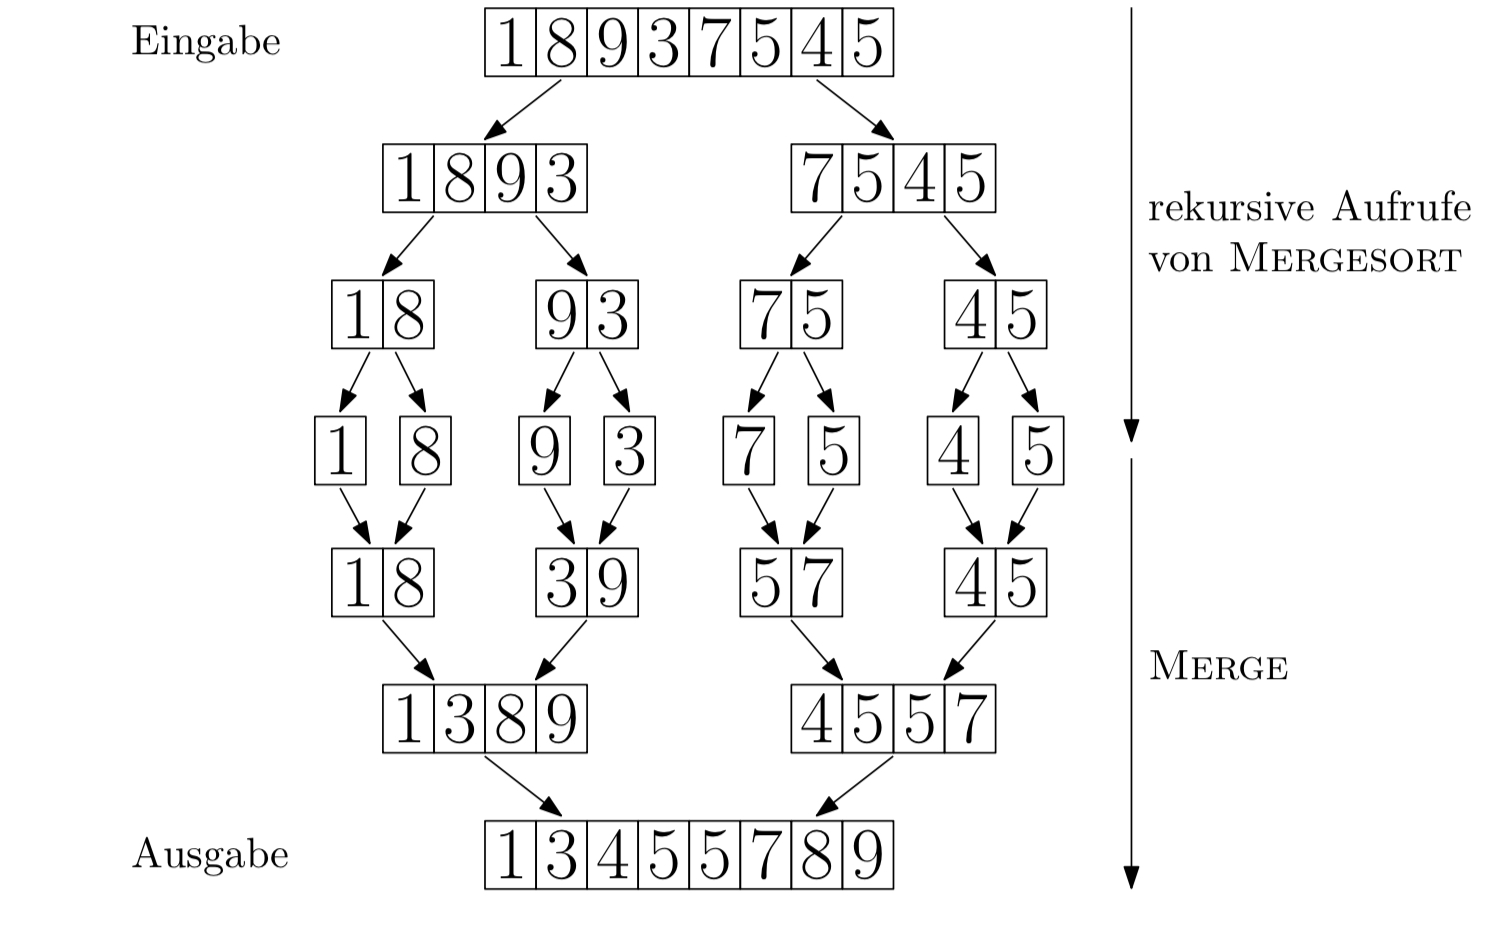
\includegraphics[width=0.8\textwidth]{images/IMG_86CA0912DB1F-1.jpeg}
	\caption{Mergesort}
	\label{fig:1}
\end{figure}
\thm{}{Die Laufzeit von Merge Sort ist in $O(n \log n)$}
\subsection{Divide-and-Conquer am Beispiel von Strassen}
\nt{Wenn man die Laufzeit von Strassen zu Simpleren Divide and Conquer Algorithmen vergleicht, wie Simple Product, ist die Laufzeit von Strassen besser}
\thm{}{Die Laufzeit von Strassen ist in $O(n^{\log_2 7})$}
\begin{myproof}
	Siehe Seite 25 skript(Kein Bock das zu Texen) folgt aber aus $T(n) = 7T(n/2) + O(n^2)$
\end{myproof}
\subsection{Master Theorem}
\thm{Mastertheorem}{Seien $a \geq 1, b > 1,$ Konstanten und sei f: $\mathbb{N} \to \mathbb{R}_{\geq 0}$ eine Funktion. Ferner sei $T: \mathbb{N} \to \mathbb{R}$ definiert durch $ T(1) = \Theta(1)$ und $$ T(n) = aT(\frac{n}{b}) + f(n)$$ für alle $n > 1$.
Die Funktion T kann wie folgt beschrieben werden:
\begin{itemize}
	\item $T(n) = O(n^{\log_b a})$ falls $f(n) = O(n^{\log_b a - \epsilon})$ für eine Konstante $\epsilon > 0$
	\item $T(n) = \Theta(n^{\log_b a} \log n)$ falls $f(n) = \Theta(n^{\log_b a})$
	\item Falls $T(n) = \Omega(n^{\log_b a + \epsilon})$ für eine Konstante $\epsilon > 0$ und falls $af(\frac{n}{b}) \leq cf(n)$ für eine Konstante $c < 1$ und alle hinreichend großen $n$, dann gilt $T(n) = \Theta(f(n))$
\end{itemize}
}
\nt{Im Prinzip werden nur die Funktionen n und $n^{\log_{b}a}$ verglichen. Im ersten Fall wächst f langsamer im zweiten gleich schnell. Verglichen zum ersten Fall führt das zu einem zusätzlichen $\log n$ führt. Im dritten Fall wächst f schneller als $n^{\log_{b}a}$, also ist die Lösung $\Theta(f(n))$}
\begin{lemma}
	Seien $a \geq 1, b > 1,$ Konstanten und sei f: $\mathbb{N} \to \mathbb{R}_{\geq 0}$ eine Funktion. Sei $T(n) = \Theta(O(n^{\log_{b}(a)})) + g(n)$ mit $g(n) \defeq \sum_{i=0}^{\log_{b}(n) - 1} a^{i}f(\frac{n}{b^{i}})$ Betrachte die Funktion beschränkt auf Werte von n mit $n = b^{j} \text{ für } j \in \mathbb{N}$.
	\begin{itemize}
		\item Falls f(n) = O($n^{\log_{b}(a) - \epsilon}$) für eine Konstante $\epsilon > 0$, dann $g(n) = O(n^{\log_{b}(a)})$
		\item Falls f(n) = $\Theta(n^{\log_{b}(a)})$, dann $g(n) = \Theta(n^{\log_{b}(a)} \log n)$
		\item Falls f(n) = $\Omega(n^{\log_{b}(a) + \epsilon})$ für eine Konstante $\epsilon > 0$ und falls $af(\frac{n}{b}) \leq cf(n)$ für eine Konstante $c < 1$ und alle hinreichend großen $n$, dann gilt $g(n) = \Theta(f(n))$
	\end{itemize}
\end{lemma}
\nt{Die Funktion g(n) ist die Summe der Kosten der rekursiven Aufrufe.\\ 
	Das Lemma beschreibt das Mastertheorem für den Fall, dass n eine Potenz von b ist. Die höhe des Rekursionbaumes beträgt $\log_{b}(n)$ Logischerweise ist die gesammte Laufzeit die Summe über alle Knoten für jedes Level, wobei sich die anzahl an Knoten mit der höhe Skaliert mit $a^{h}$ hinzu kommt dannn noch das die Kosten pro level noch mit der Summe $\sum_{i=0}^{h-1} f(\frac{n}{b^{i}})$ gegeben ist. Also ensteht daher die Formel für die gesammt Laufzeit mit $\Theta(a^{h}) + \sum_{i=0}^{h-1} f(\frac{n}{b^{i}})$}
\begin{figure}[h]
	\centering
	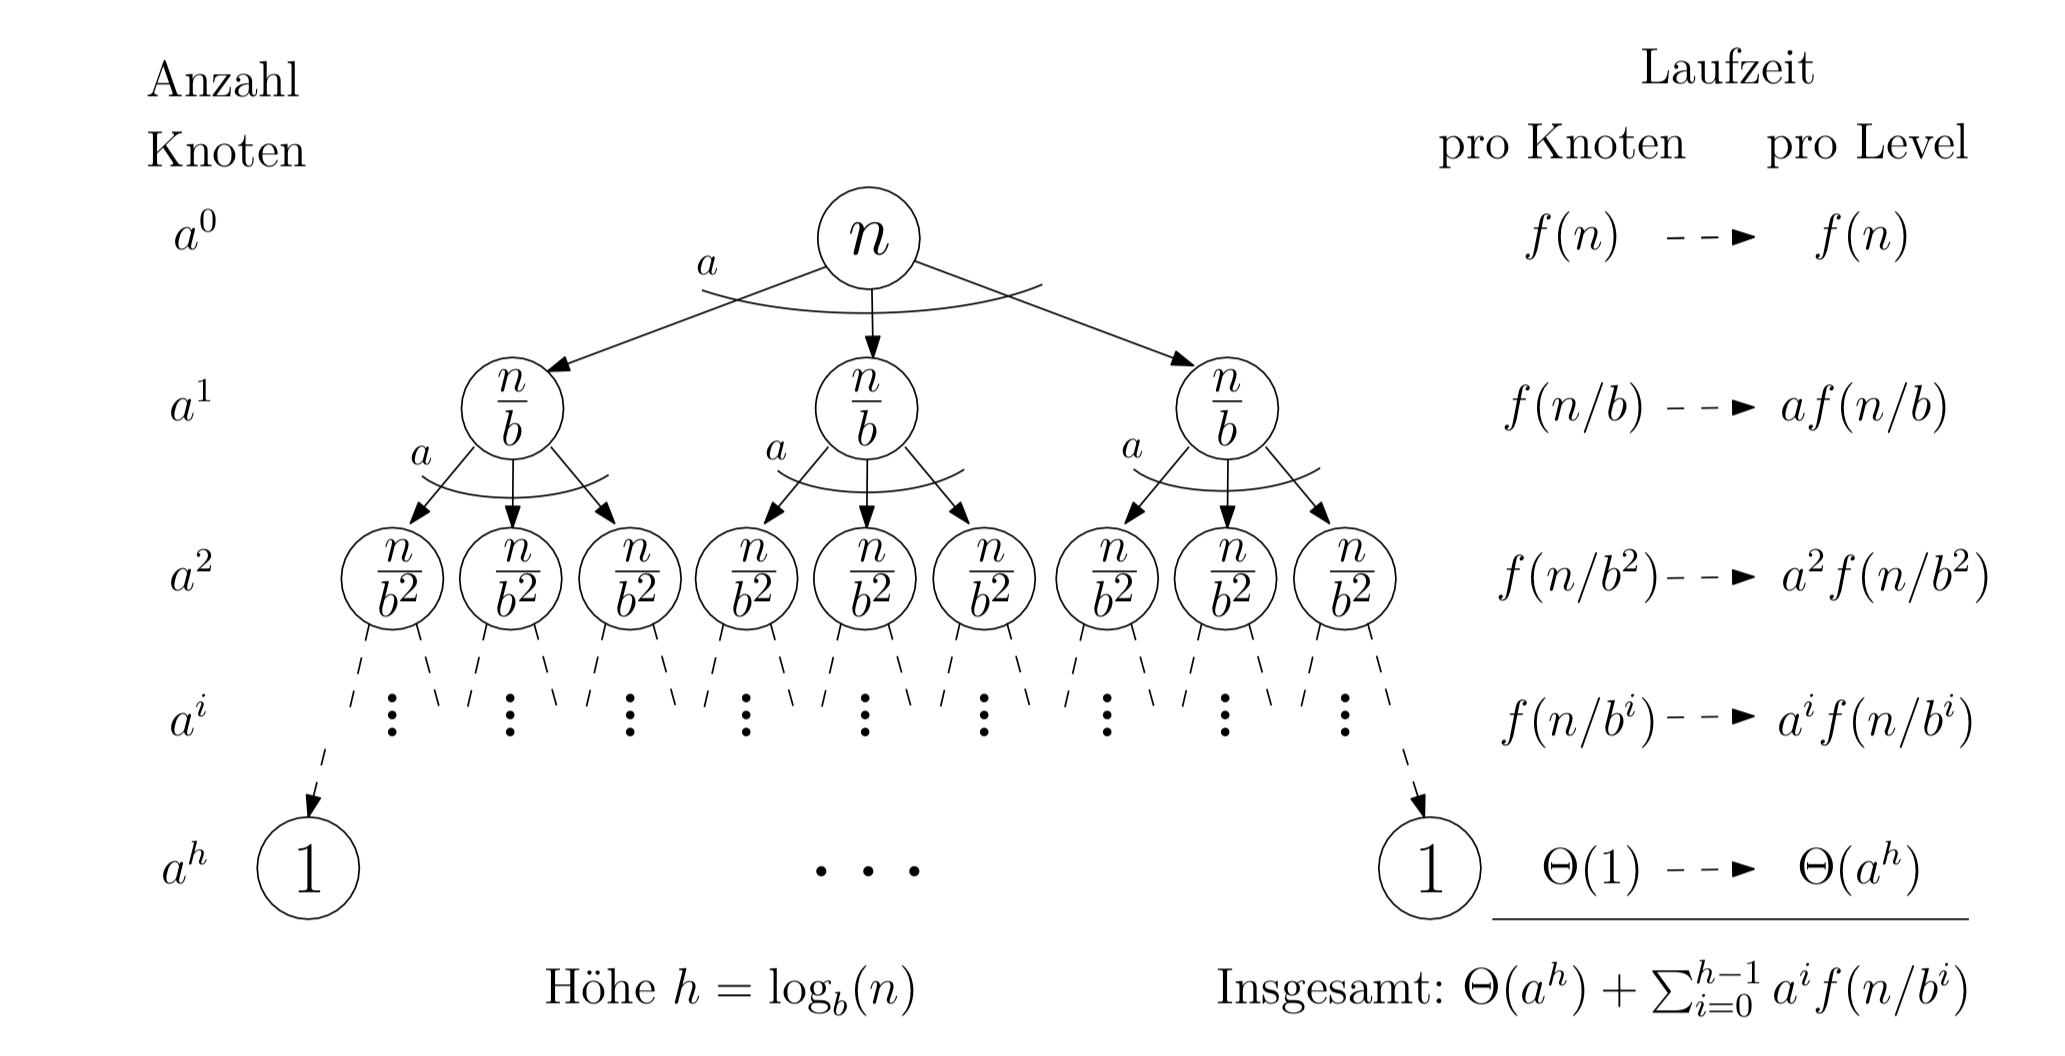
\includegraphics[width=0.8\textwidth]{images/Mastertheorem.jpeg}
	\caption{Visualized Lemma 1}
	\label{fig:2}
\end{figure}
\section{Greedy Algorithmen}
\dfn{Greedy Algorithmen}{Greedy Algorithmen sind Algorithmen die immer den besten lokalen Schritt wählen. }
\ex{Wechselgeldproblem}{Das Wechselgeldproblem stellt die Münzen schritt für schritt zusammen, die am nächsten an den Restbetrag herankommen.
Wie viel noch fehlt wird sich in der Variable $z'$ gemerkt.}
\thm{}{Der Greedy Algorithmus löst das Wechselgeldproblem optimal.(Was ist wenn die Währung doof ist, siehe nächste Note)}
\nt{Für richtige Währungen wenn man Quatsch Währungen wählt lässt sich schnell ein gegenbeispiel Konstruieren z.B. 1,3,4 jezt 6 als Betrag. Also wird halt die 4 gewählt weil die am größten ist dementsprechend wird in den nächsten 2 Schritten 2 mal die 1 gewählt, aber die 3 und 3 wären besser gewesen.}
Ich mach einfach mal nen beweis für die Vibes dazu, keine Ahnung gerade Bock drauf steht aber auch so im Skript(in Schöner siehe Seite 29).
\begin{proof}
	Sei $z \in \mathbb{N}$ ein beliebiger Betrag, welcher genau erreicht werden soll. Für $i \in M : = \{1,2,5,10,20,50,100,200\}$ mit $x_{i} \in \mathbb{N_{0}}$
	Wegen der Def von Greedy Algorithmen, das immer der Lokal beste Schritt gewählt wird folgt das die ungleichung mit $i \in M, i > 1$ gilt 
	$$ \sum_{j \in M, j < i}^{}jx_{j} < i  $$
	Das j ist hierbei die Münze die gerade betrachtet wird, diese ist immer kleiner als i, da sonst das i gewählt werden würde, was gegen die Defenition von Greedy Algorithmen verstößt, da es eine bessere Lösung gibt.\\
	Zusammen mit der Ausgangsbedingung das der zu erreichende Betrag z immer $\sum_{i \in M}^{}ix_{i}$ ist. Nun lässt sich hierdrüber folgende Induktion aufbauen.\\
	 $z = 1$ trivialerweise gilt die Aussage.\\ Die Aussage gilt für alle $z \in \mathbb{N}$ mit $z > 1$ betrachte $$ \sum_{j \in M, j < i}^{}jx_{j} < i  $$ \\ für ein $i \ maximal \leq z$ muss mindestens eine Münze vom Wert i enthalten sein, da sonst der Betrag nicht erreicht werden kann.\\
	Die Behauptung folgt auch für $z' = z - i$ da $z' \leq z$ gilt.\\ 
	Also ist die Lösung vom Greedy Algorithmus mit der Ungleichung erfüllt.\\
	Nun lässt sich Annehmen, das sich eine optimale Lösung finden lässt. Wenn man alle Münzen in M durchgeht lässt sich immer jede Münze durch eine Kombination von Münzen mit kleinerem Wert ersetzen.\\
	Formaler sei $y_{i} \in \mathbb{N}_{0}$ mit $ \sum_{i \in M} iy_{i} = z $ und kleinstmöglicher Zahl $\sum{i \in M} y_{i}$\\
	Sei die Lösung in Optimalerweise $x_{i} \in \mathbb{N}_{0}$ Zum Beispiel gilt $y_{1} \leq 1$, da zwei 1 Cent Münzen durch eine 2 Cent Münze ersetzt werden können.\\
	Daraus folgt die ungleichung $1 \cdot y_{1} < 2$\\
	Analog folgt für $y_{2}, y_{2} \leq 2$, da sich 3 2 Cent Münzen durch eine 5 Cent Münze und eine 1 Cent Münze ersetzen lassen.\\
	Daraus folgt die ungleichung $1 \cdot y_{1} + 2 \cdot y_{2} < 5$\\ $\rightarrow$ Dies gilt für alle $i \in M$
\end{proof} 
\subsection{Optimale Auswahl von Aufgaben}
\nt{Intervall Scheduling:
Jede Aufgabe hat eine Startzeit $s_{i} \geq 0$ und eine Endzeit $f_{i}$, wobei $s_{i} < f_{i}$ gilt.\\
Zudem steht ein Prozesor zur verfügung der nur eine Aufgabe gleichzeitig bearbeiten kann.\\
Die Aufgabe ist es nun eine möglichst große Teilmenge von Aufgaben zu finden, die sich nicht überschneiden.\\}
\dfn{Intervall Scheduling Formales Ziel}{Gescucht ist eine Teilmenge $S' \subseteq S$, sodass für jedes $i,j \in S'$ gilt $i \neq j$ und $[s_{i}, f_{i}) \cap [s_{j}, f_{j}) = \emptyset$}
\nt{Es liegt nahe das es einen Greedy Algorithmus gibt welcher das Problem löst(Im Skript kommen noch Algorithmen die nicht klappen)}
\begin{algorithm}[H]
\caption{Greedy Ende}
$S^{*}$ = $\emptyset$\\
\While{$S \neq \emptyset$}{
	\text{Wähle die Aufgabe i mit dem frühesten Ende}\\
	$S^{*} = S^{*} \cup \{i\}$\\
	$S = S \setminus \{i\}$ \text{Keine Ahnung nicht im Skript aber kommt mir logisch vor}\\ 
	\text{Entferne alle Aufgaben die sich mit i überschneiden}

}
\end{algorithm}
Für den Beweis von den Algorithmus wird folgendes Lemma benötigt.
\mlenma{}{Es sei S eine Menge von Aufgaben und es sei $i \in S$ eine Aufgabe mit dem frühesten Ende. Dann gibt es eine Optimale Auswahl $S' \subseteq S$ von paarweise nicht kollidierenden Aufgaben mit $i \in S'$}
\nt{Das Lenma sagt basically nur aus das es eine optimale Lösung gibt.}
\begin{proof}
	Genauer Beweis im Skript seite 32. Aber man definiert sich eine Optimale Menge $S^{*}$ in diese fügt man dann eine Aufgabe i ein. Die Menge $S^{*}$ ist dann immer noch optimal und es gibt keine Überschneidungen, da i vor oder gleich mit j der vorher kürzesten Aufgabe aufhört. j hat sich halt obviously auch nicht überschnitten, weil dann wär es nicht optimal gewesen. 
\end{proof}
\thm{}{Der Algorithmus GreedyEnde wählt für jede Instanz eine größtmög-
liche Menge von paarweise nicht kollidierenden Aufgaben aus.}
\begin{proof}
	Lässt sich recht entspannt über ne invariante Zeigen:\\
	In Zeile 2 gilt immer das $S^{*}$ sich zu einer optimalen Lösung erweitert.\\
	In der ersten Iteration gilt die Invariante, da \( S^* \) leer ist und \( S \) noch alle Aufgaben enthält. Sei nun die Invariante zu Beginn eines Schleifendurchlaufs erfüllt. Dann gibt es eine optimale Auswahl \( \hat{S} \subseteq S^* \cup S \) von Aufgaben, die alle Aufgaben aus \( S^* \) und gegebenenfalls zusätzliche Aufgaben aus \( S \) enthält. Außerdem kollidieren Aufgaben aus \( S^* \) nicht mit Aufgaben aus \( S \). Das heißt, bei der Frage, welche Aufgaben aus \( S \) den Aufgaben aus \( S^* \) noch hinzugefügt werden müssen, um eine optimale Auswahl \( \hat{S} \) zu erhalten, spielen die Aufgaben aus \( S^* \) keine Rolle. Die Menge \( \hat{S} \setminus S^* \) dieser Aufgaben ist eine größtmögliche Teilmenge von paarweise nicht kollidierenden Aufgaben aus \( S \). Gemäß Lenma 2.2.1 existiert eine solche Menge, die die Aufgabe \( i \in S \) mit dem frühesten Fertigstellungszeitpunkt \( f_i \) aller Aufgaben aus \( S \) enthält. Genau diese Aufgabe fügt der Greedy-Algorithmus am Ende der Menge \( S^* \) hinzu. Anschließend werden aus \( S \) alle Aufgaben entfernt, die mit dieser Aufgabe \( i \) kollidieren. Dies garantiert zusammen, dass auch am Anfang der nächsten Iteration die Invariante wieder erfüllt ist.
\end{proof}
\dfn{Laufzeit Greedy Ende}{Die Laufzeit des Algorithmus GreedyEnde beträgt $O(n \log n)$, wobei $n = |S|$ die Anzahl der Aufgaben in der Eingabe bezeichnet. Sind die Aufgaben bereits aufsteigend nach ihrem Fertigstellungszeitpunkt sortiert, so beträgt die Laufzeit O(n).}
\nt{Es läuft halt n mal durch und man kann es in $O(n \log n)$ sortieren.}
\subsection{Rucksackproblem mit Teilbaren Aufgaben}
Das Rucksack, wie wir es Behandeln (anscheinend kommt mehr in Algo 2) besteht aus einer Menge von Objekten $O = \{1, \dots, n\}$, wobei jedes Objekt $i \in O$ ein Gewicht $w_{i} \in \mathbb{N}$ und einen Nutzen $p_{i} \in \mathbb{N}$ besitzt.\\
Es soll eine Teilmenge der Objekte gefunden werden, die in den Rucksack passt und unter dieser Bedingung maximalen Nutzen besitzt.
Jetzt wo es ein bisschen anders ist: \\ Wir dürfen das Objekt Teilen für den maximalen Nutzen.

\begin{algorithm}[H]
\caption{Greedy Rucksack}
Sortiere die Objekte nach dem Nutzen pro Gewicht $p_{i}/w_{i}$ in absteigender Reihenfolge.\\
\For{int i = 1; i $\leq$ n; i++}{x[i] = 0;}
int i = 1;\\
\While{$t>0$ and $i\leq n$}{
	\If{$t \geq w_{i}$}{
		$x_{i} = 1$\\
		$t = t - w_{i}$
	}
	\Else{x[i] = t/w[i], t = 0\\}
	i++;
}
\Return{$x_{1}, \dots, x_{n}$}
\end{algorithm}
\thm{}{Der Algorithmus GreedyRucksack liefert für jede Instanz eine optimale Lösung in $O(n \log n)$ Zeit.}
\begin{proof}
	Zur Laufzeit: Greedy Rucksack wird von den Sortieren Dominiert, dies läuft über Merge-Sort in $O(n \log n)$. Die Schleifen können jeweils nur n mal durchlaufen, was die laufzeit von $O(n \log n)$ zeigt.\\
	Zur Korrektheit: Da die Lösung trivial ist, wenn alle Objekte in den Rucksack passen wird im folgenden nur der andere Fall betrachtet mit $t < \sum_{i=1}^{n} w_{i}$.\\
	Es gibt nun ein $i \in \{1, \dots, n\}$ mit $x_{1} = \dots = x_{i-1} = 0 $ $x < 1 $ und $x_{i+1} = \dots = x_{n} = 0$\\
	Greedy Rucksack füllt natürlich auch den Rucksack. Jede Optimale Lösung muss den Rucksack auch ausfüllen, das heißt es gilt $\sum_{i=1}^{n} x_{i}^{*} w_{i} = t$.\\
	Es wird nun gezeigt, dass sich die Lösung von $x^{*}$ in die Lösung x von Greedy Rucksack umwandeln lässt ohne die Nutzen zur veringern.\\
	Jetzt wird der kleinste Index i genommen $x_{i}^{*} < 1$ und $x_{i+1}^{*} = \dots = x_{n}^{*} = 0$. Hier gilt jetzt $x^{*} = x$ muss mir nochmal anschauen warum.TODO
	Es gibt einen Index $j > i$ mit $x_{j}^{*} > 0$. Sei j der größte solcher Indexe. Die j lassen sich jetzt reduzieren während man das i gegenscaled. Wegen der Effizienz von i welche mindestens die von j ist verändert sich nicht der Nutzen
\end{proof}
Da die Lösung zwar immer Korrekt ist aber vergleichsweise Langsam wird jetzt ein Appromixativer Algorithmus eingeführt.
\begin{algorithm}[H]
\caption{Approximative Greedy Rucksack}
Berechne mit Int Greedy Rucksack eine Lösung $x_{1}^{*}, \dots, x_{n}^{*}$\\
j = argmax\{$p_{i}$\}, $ i \in \mathbb{N}$\\
\If{$\sum^{n}_{i = 1} p_{i}x_{i}^{*} \geq p_{j}$}{
	\Return{$x^{*}$}
}
\Else{
	\Return{$x' = (x'_{1} \dots x'_{n})$ mit $x'_{1} = \begin{cases}
		0 \ \text{falls} \ i \neq j \\
		1 \ \text{falls} \ i = j 
		\end{cases}$
		 }
}
\end{algorithm}
\thm{}{ Der Algorithmus Approximative Greedy Rucksack berechnet auf jeder Eingabe für das Rucksackproblem mit n Objekten in Zeit $O(n \log n)$ eine gültige ganzzahlige Lösung, deren Nutzen mindestens halb so groß ist wie der Nutzen einer optimalen ganzzahligen Lösung.}

\section{Dynamische Programmierung}
\subsection{Einführung und einfaches Beispiel Fibonacci}
Bei Fibonacci lässt sich folgende Funktion aufstellen: \\
$f_{n} = 
\begin{cases}
	0 \ \ \text{falls} \ n = 0 \\
	1 \ \ \text{falls} \ n = 1 \\
	f_{n-1} + f_{n-2} \ \ \text{falls} \ n \geq 2 \\
\end{cases}$

Daraus folgt der Algorithmus

\begin{algorithm}[H]
\KwIn{int n}
\caption{Fibonacci-Rek}
\If{n == 0}{\Return{0}}
\If{n == 1}{\Return{1}}
\Else{\Return {Fibonacci-Rek(n-1) +Fibonacci-Rek(n-2) } }

\end{algorithm}

\subsection{Berechnung optimaler Zuschnitte}
Ok, wir lernen jetzt wie man Holz Dealer wird.\\
Die Eingabe hier ist $ n \in \mathbb{N}  $ Wenn wir ein Brett in 5 Teile Zerlegen können wir jetzt alel Kombinationen durchgehen und schauen was am besten ist.\\
Das ist ein bisschen zu schlecht wegen exponentieller Laufzeit, deswegen wird Dynamisch Programmiert.
Für $ i \in \{1, \dots , n \}$ wird der maximale Erlös $R_{i}$ für ein Brett der Länge i berechnet.
Das berechnen von $R_{i}$ wird als Teilproblem bezeichnet.
Die Lösung des Gesamtproblems ist dann $R_{n}$
Es gilt natürlich $R_{1} = p_{1}$, da wir ein brett der länge 1 nicht zerlegen können\\
\mlenma{}{Für $ i \in \{1, \dots , n \}$ gilt $R_{i} = max \{p_{j} + R_{i-j} , j \in \{1, \dots , n \}$}

\begin{algorithm}[H]
\caption{Optimaler Zuschnitt}
\KwIn{int n}
\KwOut{int $R_{n}$}
$R_{0} = p_{0}$\\
\For{i = 1; $i \leq n$; i++}{
	$R_{i} = -1$
	\For{j=1; $j \leq i$; j++}{
		$R_{i} = max\{R_{i}, p_{j} + R_{i-j}\}$
	}

}
\Return{$R_{n}$}
\end{algorithm}
\thm{}{Der Algorithmus berechnet in $O(n^{2})$ Zeit den optimalen Erlös für ein Brett der Länge n.}
\subsection{Rucksackproblem}
\end{document}
